	\chapter{Completezza delle funzioni ricorsive parziali}
	
	Faremo vedere che la famiglia di funzioni ricorsive parziali, è uguale alla funzioni URM-calcolabili.
	
	\section{Funzioni ricorsive parziali}
	La famiglia delle funzioni ricorsive parziali è quella delle funzioni definibili a partire dalle funzioni iniziali e con
	\begin{itemize}
		\item Composizione
		\item Ricorsione primitiva
		\item Minimalizzazione (non limitata)
	\end{itemize}
	
	Il nostro obiettivo sarà dimostrare che famiglia di funzioni ricorsive parziali, è uguale alla funzioni URM-calcolabili. Con la tesi di Church, vedremo come parleremo di funzioni calcolabili, e non solo URM-calcolabili.
	
	\section{Funzione di Ackermann}
	La funzione di Ackermann permette di esplicitare il limite delle funzioni ricorsive primitive. Il motivo per cui non può essere espressa tramite ricorsione primitiva, è la doppia ricorsione. Anche la funzione dei numeri di Fibonacci può essere ricondotta ad una forma primitiva ricorsiva, ma questa funzione no.
	
	$$
	\psi(x,y)=
	\begin{cases}
		\psi (0, y) = \begin{cases}
			1 & \text{se } y=0 \\
			2 & \text{se } y=1 \\
			y+2 & \text{se } y>1
		\end{cases}
		& \text{se } x=0 \\[14pt]
		\psi (x, 0) = 1 & \text{se } x\geq 1,\; y=0 \\[6pt]
		\psi(x+1,y+1) = \psi(x,\psi(x + 1,y)) 
		& \text{se } x\geq 1,\; y\geq 1
	\end{cases}
	$$
	
	per facilitare, cambiamo notazione. $\psi_x(y) \equiv \psi(x,y)$.
	
	$$
	\psi_x(y)=
	\begin{cases}
		\psi_0 (y) = \begin{cases}
			1 & \text{se } y=0 \\
			2 & \text{se } y=1 \\
			y+2 & \text{se } y>1
		\end{cases}
		& \text{se } x=0 \\[14pt]
		\psi_x (0) = 1 & \text{se } x\geq 1,\; y=0 \\[6pt]
		\psi_{x+1}(y+1) = \psi_x(\psi_{x+1}(y)) 
		& \text{se } x\geq 1,\; y\geq 1
	\end{cases}
	$$
	
	osserviamo che $\psi_{x+1}(y+1) = \psi_x(\psi_{x+1}(y)) = \psi_x^{(y+1)}(1)$. In generale dimostrare la calcolabilità di questa funzione non è facile.
	\subsection{Dimostrazione calcolabilità di $\lambda y.\psi_x(y)$}
	Faremo vedere per induzione su $x$ che la restrizione (unaria) $\lambda y.\psi_x(y)$ è calcolabile e totale. Osserviamo che non stiamo andando a valutare la funzione al variare di $x$, ma stiamo valutando su valori fissati di $x$.
	
	\begin{itemize}
		\item Caso base: $\lambda y.\psi_0(y)$. Questo termine è già presente nella definizione per casi.
		
		$$
		\psi_0(y) = \begin{cases}
			1 & \text{se } y=0 \\
			2 & \text{se } y=1 \\
			y+2 & \text{se } y>1
		\end{cases}
		$$
		\item Passo induttivo: l'ipotesi induttiva è che $\psi_x(y)$ sia calcolabile e totale. Si osservi quindi che la funzione $\psi_{x+1}$ può essere definita sulla seguente ricorsione primitiva (su $y$), in termini di $\psi_x$:
		
		$$
		\begin{cases}
		\psi_{x+1}(0) = 1\\
		\psi_{x+1} (y+1) = \psi_x(\psi_{x+1}(y))
		\end{cases}
		$$
	\end{itemize}
	
	pertanto, per induzione, $\psi_{x+1}$ è calcolabile e totale. Il fatto che questa funzione sia calcolabile per $x$ fissati, non significa che la funzione di Ackermann sia calcolabile.
	
	\begin{figure}[tbph]
		\centering
		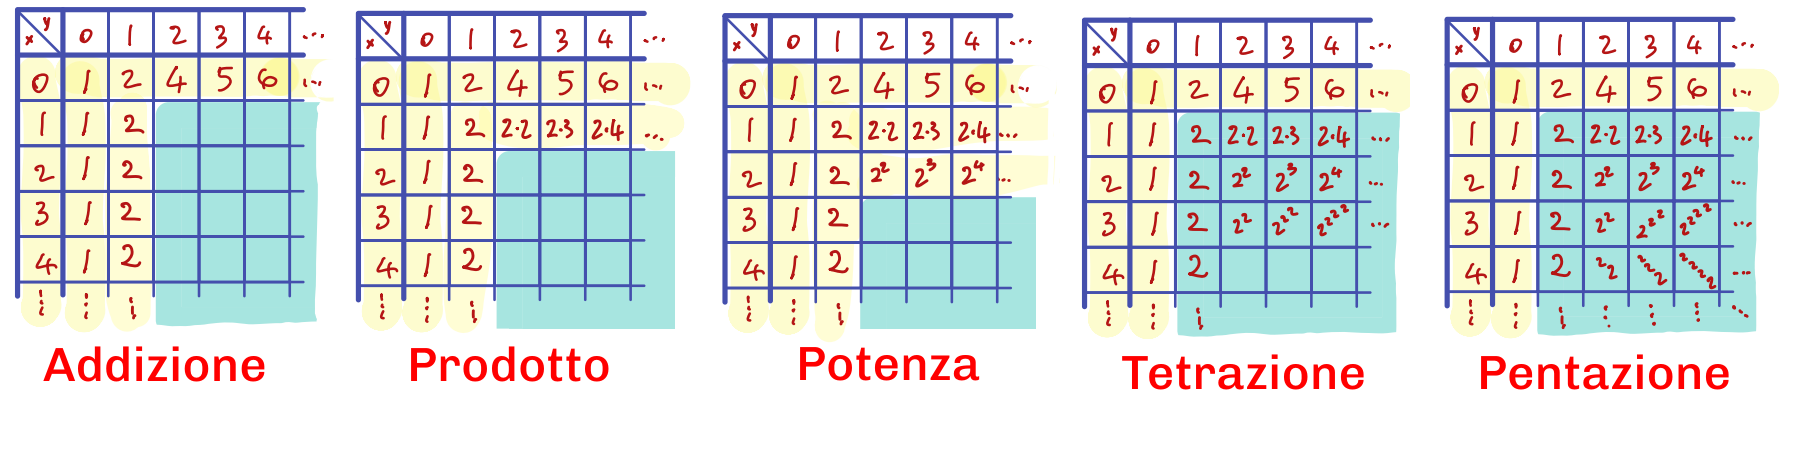
\includegraphics[width=1\linewidth]{images/ackermann}
	\end{figure}
	
	
	\subsection{Calcolabilità della funzione di Ackermann}
	Questa è la parte più difficile della dimostrazione.
	
	
	\paragraph{Triple} Intendiamo caratterizzare insiemi finiti $S$ di triple $(x,y,z) \in\mathbb{N}$ tali che, $\forall (x,y,z)\in \S$:
	\begin{itemize}
		\item $z=\psi(x,y)$
		\item $S$ contiene \textbf{tutte} le triple $(\overline{x},\overline{y}, \psi(\overline{x},\overline{x}))$ necessarie al calcolo di $\psi(x,y)$.
	\end{itemize}
	
	questi insiemi devono inoltre essere \textbf{validi}.
	
	\paragraph{Insiemi validi} Un insieme di triple $S$ è detto valido se le seguenti condizioni sono soddisfatte:
	\begin{itemize}
		\item se $(0,y,z) \in S$, allora $z = \begin{cases}
			1 & \text{se } y=0 \\
			2 & \text{se } y=1 \\
			y+2 & \text{se } y>1
		\end{cases}$.
		\item se $(x,0,z) \in S$, allora $z = 1$.
		\item se $(x+1,y+1,z) \in S$, allora $\exists u \in \mathbb{N}: \ (x+1, y, u), (x, u, z)$.
		
	\end{itemize}
	
	Osserviamo che $
	\psi(x+1,y+1)=
	\psi\big(\overbrace{x,\underbrace{\psi(x+1,y)}_{w}}^{z}\big)
	$. Un insieme finito di triple $S$ è detto \textbf{valido rispetto alla coppia} $(x,y) \in \mathbb{N}^2$ se
	\begin{itemize}
		\item $S$ è valido.
		\item $\exists u \in \mathbb{N} : (x,y,u) \in S$.
	\end{itemize}
	
	Possiamo poi definire un buon ordinamento $<_{\mathrm{lex}} \text{ su } \mathbb{N}\times\mathbb{N}$.
	$$
	(x,y) <_{\mathrm{lex}} (x',y')
	\;\Longleftrightarrow\;
	\big(x < x'\big) \;\vee\; \big(x = x' \land y < y'\big).
	$$
	
	\paragraph{Fatto 1} Se $S$ è valido, allora $\forall (x,y,z) \in S \Rightarrow z = \psi(x,y)$. Si dimostra per assurdo.
	
	{\huge TODO}
	
	\paragraph{Fatto 2} $\forall (x,y) \in \mathbb{N}^2, \exists S$ finito valido per $(x,y)$. Si dimostra per assurdo.
	
	{\huge TODO}
	
	\paragraph{Passo finale della dimostrazione}
	Una tripla $(x,y,z)$ può essere codificata in un singolo numero positivo $u = 2^x3^y5^z$, mentre un insieme finito di numeri positivi, e quindi di triple, può essere codificato in un singolo numero $v = p_{u_1}p_{u_2}\dots p_{u_k}$. Il set di triple codificato da $v$ è indicato con $S_v$.
	 
	Quindi, $(x,y,z) \in S_v \Leftrightarrow p_{2^x3^y5^z} \text{ divide }v$. Essendo questa una mutua implicazione, la decidibilità di un predicato implica la decidibilità dell'altro. Definiamo quindi la funzione
	
	$$
	R(x,y,v) \equiv \text{ "$v$ codifica un insieme valido di triple e $\exists z < v ((x,y,z) \in S_v)$"}.
	$$
	
	Essendo questo un predicato decidibile, è calcolabile anche la funzione
	
	$$
	f(x,y) = \mu v R(x,y,v)
	$$
	
	Ne consegue che la funzione di Ackermann è calcolabile tramite
	$$
	\psi(x,y) = \mu z ((x,y,z) \in S_{f(x,y)})
	$$